\documentclass[aspectratio=169]{beamer}

% \renewcommand{\textSupervisors}    {Supervisors}

\usetheme{vega}

\title{Optimal execution problem in Obizhaeva--Wang framework}
\subtitle{SRG Market microstructure}
\author{Vsevolod Zaostrovsky, Peter Shkenev}
\institute{Vega Institute Foundation}
\supervisor{Anton Belyakov, Alexey Savin}
% \date{August 21 -- 28, 2022}

\usepackage[]{lipsum}
\begin{document}
\maketitle

\begin{frame}{Optimal execution problem}
    Task: we want to buy or sell a big amount of asset. \par
    \begin{figure}
        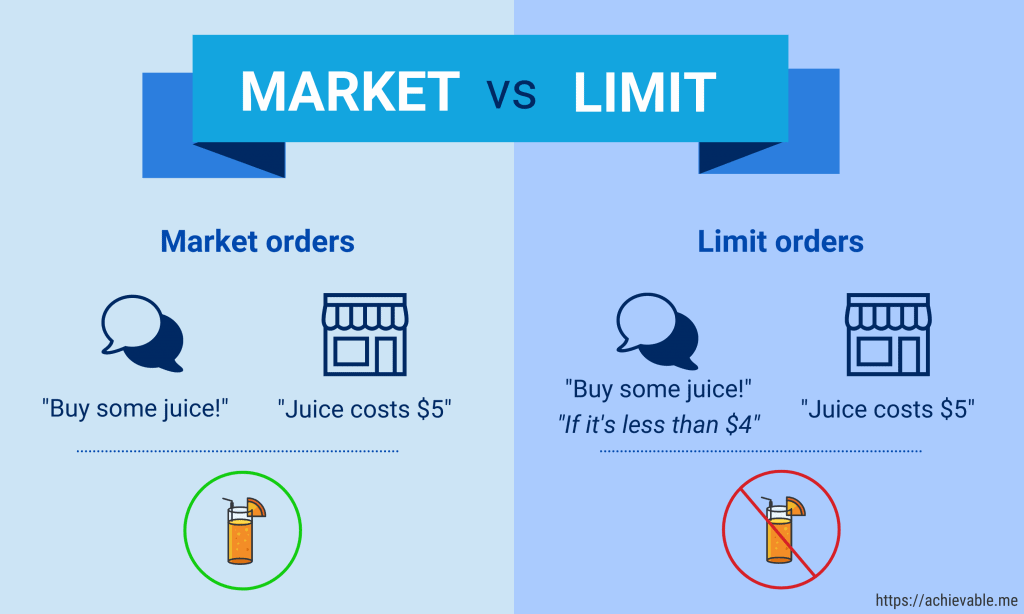
\includegraphics[scale=0.23]{figs/market-vs-limit-1024x614.png}
        \caption{The difference between market order and limit order}
        \label{fig:mvslim}
    \end{figure}
    So, let's go to the exchange and just buy as many assets as needed!

\end{frame}

\begin{frame}{The structure of LOB and problems of such approach}
    \begin{figure}
        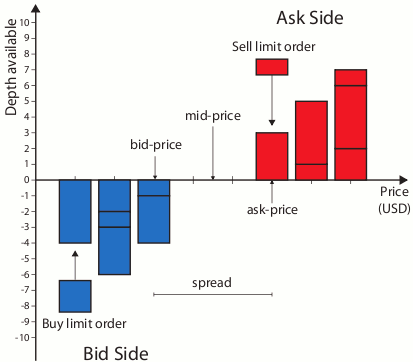
\includegraphics[scale=0.45]{figs/Graphical-representation-of-the-Limit-Order-Book.png}
        \caption{The structure of LOB}
        \label{fig:mvslim}
    \end{figure}

\end{frame}

\begin{frame}{Time Weighted Average Price}
    \begin{figure}
        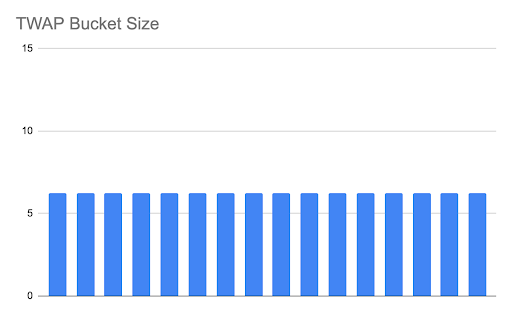
\includegraphics[scale=0.55]{figs/TWAP_Order_Type.png}
        \caption{TWAP strategy}
        \label{fig:mvslim}
    \end{figure}


\end{frame}


\begin{frame}{Resilency}
    \begin{figure}
        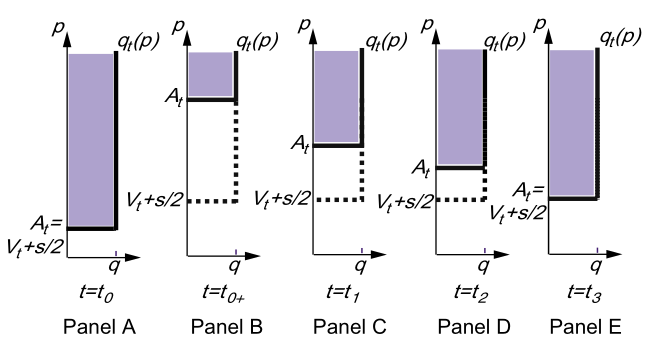
\includegraphics[scale=0.45]{figs/OWpicture.png}
        \caption{The demonstration of resiliency}
        \label{fig:mvslim}
    \end{figure}

\end{frame}

\begin{frame}{Formalization of the problem in the discrete time}
    \begin{align} \label{optexp}
        J_0 &= \min _{\{x_0 \cdots x_N \}} E_0 \left[ \sum _{n=0}^N [A_{t_n} + x_n /(2q)] x_n\right], 
        % A_{t_n} &= F_{t_n} + \lambda (X_0 - X_{t_n}) + s/2 + \sum _{i=0}^{n-1} x_i \kappa e^{- \rho \tau (n - i)},
     \end{align}
     
    where:
    \begin{itemize}
     \item The trader has to buy $X_0$ units of a security over a fixed time period $[0,T]$; 
     \item $x_{n}$ 
     is the market order size at $t_n = \tau n$, where $\tau = T / N$ and $\sum x_n = X_0$;
    %  \item $X_{t_n} := X_0 - \sum _{t_k < t_n} x_{t_k}$;
     \item $A_{t_n}$ is an ask price at $t_n$; 
    %  \item $V_{t_n} = \frac{A_{t_n} + B_{t_n}}{2}$ 
    %  is the mid-quote price; 
    %  \item $s$ is the bid–ask spread;
    %  \item $F_t$ is the fundamental value of the security;
     % \item $q(P)$ --- the density of limit orders to sell at price $P$.
     \item $q$ is a LOB density. 
    \end{itemize}

\end{frame}


\begin{frame}{The limit of the optimal execution strategy in OW framework}
    
    \begin{theorem}
        As $N \rightarrow \infty$, the optimal execution strategy becomes:
        \begin{align*}
            & \lim _{N \rightarrow \infty} x_0 = x_{t = 0} = \frac{X_0}{\rho T + 2}, \\
            & \lim _{N \rightarrow \infty} x_n / (T/N) = \dot X _t = \frac{\rho X_0}{\rho T + 2}, \;\;\;\;\;\; t \in (0, T), \\
            & \lim _{N \rightarrow \infty} x_n / (T/N) = x_{t=T}=  \frac{X_0}{\rho T + 2},  \\
        \end{align*}
        where $x_0$ is the trade at the beginning of trading period, $x_N$ is the trade at the end of trading
        period, and $\dot X _t$ is the speed of trading in between these trades.
    \end{theorem}

\end{frame}

\begin{frame}{Our methodology to fit parameters?}
    We chose regression to find parameters:                                                                                                                                                                                                                                                                                                                                                                                       
            \begin{equation*}
                \frac{\Delta A_{k+2}}{\Delta t_{k+2}} - \frac{\Delta A_{k+1}}{\Delta t_{k+1}} 
        = - \rho \Delta A_{k+1} + \rho \lambda x_{k+1} + (\kappa + \lambda) (\frac{x_{k+2}}{\Delta t_{k+2}} - \frac{x_{k+1}}{\Delta t_{k+1}}).
            \end{equation*}

        Where all the information needed can be extracted from the l3 data: 
        \begin{itemize}
            \item $\Delta A_{k}$ is an ask change after execution of the limit order with the depth $x_k$.
            \item $\Delta t_{k}$ is a time between $k$ and $k + 1$ orders of dataset.
        \end{itemize}
\end{frame}

\begin{frame}{Research plan}
    \begin{itemize}
        \item Develop methodology for fitting OWM parameters and use it to get optimal execution strategy. 
        \item Compare different approaches of measuring resiliency on l3 data.
        \item Compare discrete and limit OW execution strategies.
        \item Propose a backtest procedure for the optimal execution algorithm, implement it, and compare the algorithm with TWAP
        on real market data.
    \end{itemize}
\end{frame}

\end{document}